\chapter{Deep Learning}
\thispagestyle{fancy}
\label{chap:Deep Learning}

\noindent
Deep Learning ist ein Teilbereich des \ac{ML}. \ac{ML}-Algorithmen analysieren Daten automatisiert mittels mathematischer Methoden der Mustererkennung. \ac{DL}-Algorithmen bedienen sich hingegen vielschichtiger und hoch parametrisierter neuronaler Netze, um dem menschlichen Gehirn bestmöglich nachzuempfinden \cite[S.~455-457]{KHA19}. Dabei werden sehr große Datenmengen verarbeitet und analysiert, um einen Lerneffekt zu erzielen. Neben einer Eingabe- und einer Ausgabeschicht sorgen insbesondere die verborgenen Schichten für die prädizierte Tiefe. Hier werden Informationen weiterverarbeitet, abstrahiert und reduziert \cite[S.~131]{ZHA20}. Die potenziellen Einsatzmöglichkeiten gehen über die der \ac{ML}-Algorithmen hinaus. Der Aufbau neuronaler Netze sowie deren Funktionsweise und ausgewählte Architekturen werden in diesen Kapitel thematisiert. Hyperparameter und \ac{TL} schließen sich an.


\section{Neuronale Netze}
\noindent
Um den Aufbau und die Funktionsweise neuronaler Netze verstehen zu können, bedarf es zunächst der Beschreibung von Neuronen. Diese können im biologischen Sinne als Schalter verstanden werden, welche verschiedene Signale empfangen können und aktiviert werden, sobald genug Signale registriert wurden. Diese Aktivierung sendet folglich weitere Signale an andere Neuronen, wie \autoref{pic:ArtificialNeuron} im technischen Sinne exemplarisch skizziert \cite[S.~42]{KRI05}. Hierfür werden Aktivierungsfunktionen benötigt, welche die gewichteten Eingangssignale in ein Ausgangssignal konvertieren. Sie ermöglichen es, nicht-lineare Zusammenhänge zwischen den Eingangs- und den Ausgangsdaten herzustellen \cite[S.~134]{ZHA20}.\\

\noindent
Die elementarste Form neuronaler Netze wird \ac{MLP} genannt. \ac{MLP} bestehen aus mehreren Schichten, deren Neuronen jeweils vollständig mit den Neuronen der umliegenden Schichten verbunden sind \cite[S.~131]{ZHA20}. Der Verständlichkeit halber veranschaulicht \autoref{pic:MultiLayerPerceptron} einen solchen Aufbau mit nur einer verborgenen Schicht (engl. Hidden Layer), welche aus fünf Neuronen besteht. Dabei zeichnen sich vollvermaschte Schichten (engl. Fully Connected Layer oder Dense Layer) dadurch aus, dass alle Neuronen mit allen Inputs und Outputs verbunden.\\

\begin{figure}[h!]
  \centering
  \fbox{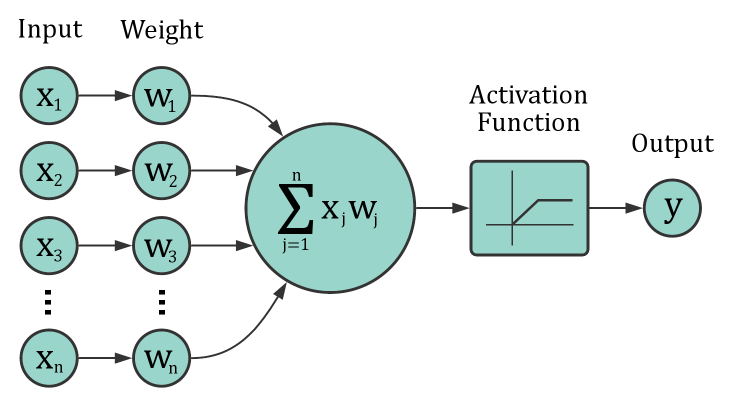
\includegraphics[width=0.55\linewidth]{./source/images/artificialneuron.png}}
  \caption{Aufbau eines künstlichen Neurons \cite{MCC20}.}
  \label{pic:ArtificialNeuron}
\end{figure}

\begin{figure}[h!]
  \centering
  \fbox{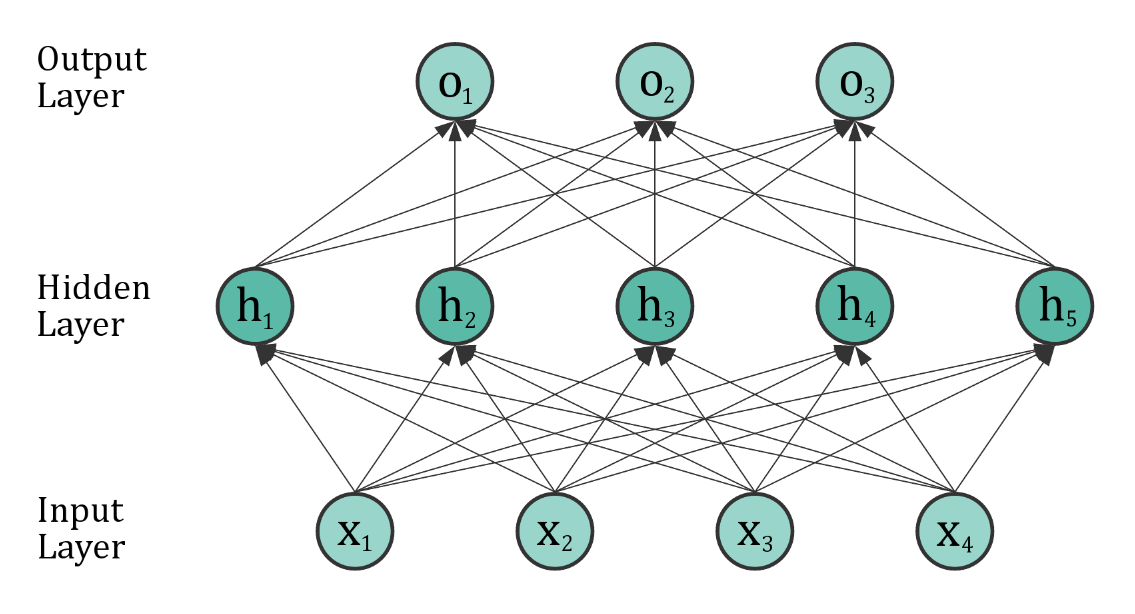
\includegraphics[width=0.6\linewidth]{./source/images/multilayerperceptron.png}}
  \caption{Aufbau eines MLP \cite[S.~388]{RAS19}.}
  \label{pic:MultiLayerPerceptron}
\end{figure}

\noindent
Ziel der hoch parametrisierten neuronalen Netze ist es, komplexe Funktionen hohen Grades bestmöglich zu approximieren und so verschiedenste Probleme zu lösen. Der anvisierte Lerneffekt wird mithilfe des sogenannten Backpropagation-Algorithmus erreicht. Hierbei werden Eingangsdaten zunächst vorwärts durch ein neuronales Netz hindurch propagiert. Mithilfe einer Fehlerfunktion wird sodann die erwartete mit der tatsächlichen Ausgabe verglichen und bewertet. Demzufolge sind gelabelte Daten erforderlich, um das hier beschriebene überwachte Training (engl. Supervised Learning) ausführen zu können \cite[S.~3]{RAS19}. Über das Gradientenverfahren werden die Fehler nun rückwärts durch das neuronale Netz propagiert und somit die Gewichte in den Neuronen angepasst, insbesondere in den verborgenen Schichten. Ziel ist die Minimierung der Fehlerfunktion und letztlich die Optimierung der durch das neuronale Netz approximierten Funktion. \autoref{pic:SupervisedLearning} verdeutlicht nochmals die Funktionsweise von überwachten Lernalgorithmen, welche in Folge eines Trainingsprozesses unbekannte Daten verarbeiten können \cite[S.~140, 169]{ZHA20}.\\

\begin{figure}[h!]
  \centering
  \fbox{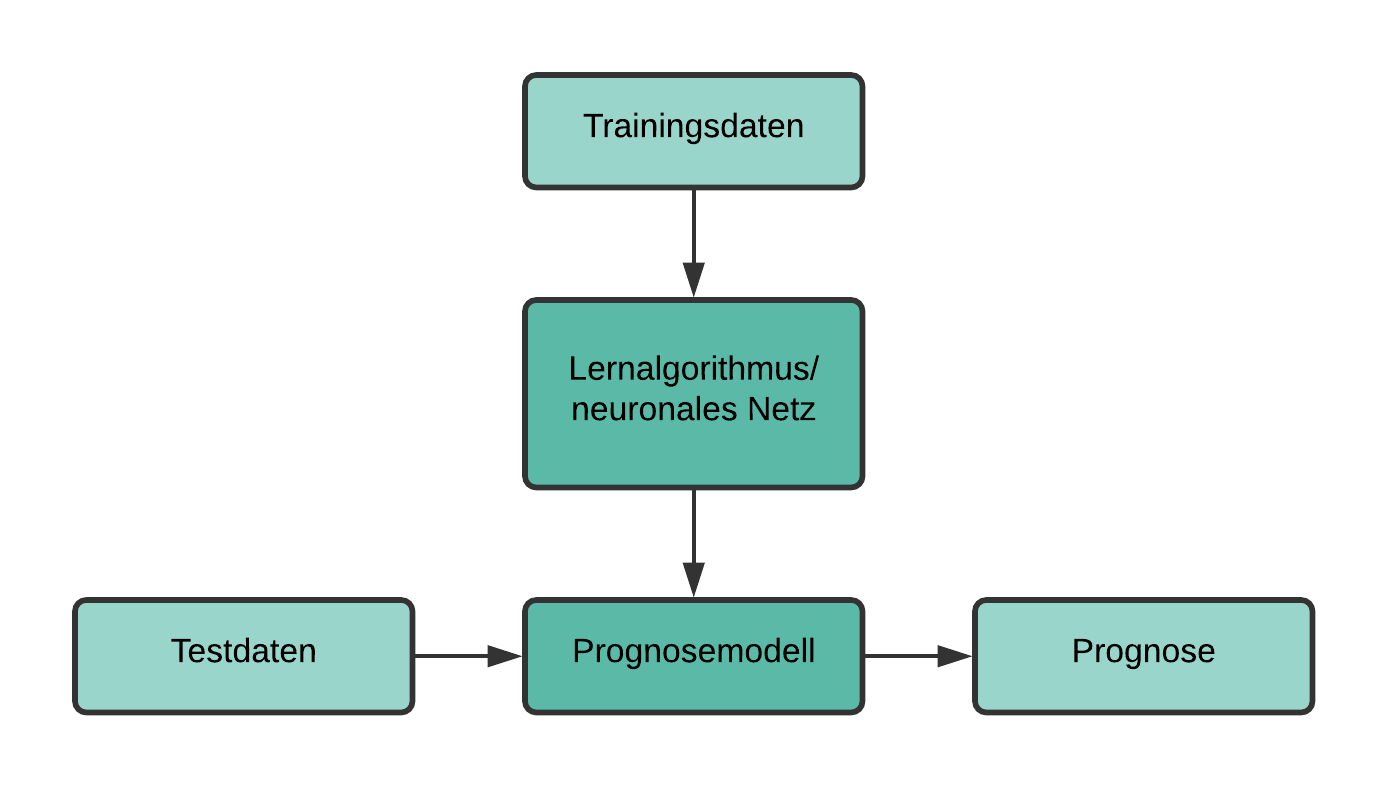
\includegraphics[width=0.7\linewidth]{./source/images/supervisedlearning.png}}
  \caption{Supervised Learning \cite[S.~3]{RAS19}.}
  \label{pic:SupervisedLearning}
\end{figure}

\noindent
Der Trainingsprozess erfolgt optimalerweise über mehrere sogenannte Epochen. Hier werden dem neuronalen Netz verschiedene Eingangsdaten zugeführt und beidseitige Propagationen ausgeführt. Wichtig ist dennoch, kein Overfitting beziehungsweise Underfitting zu erzeugen. Dies würde bedeuten, dass das trainierte Modell zu sehr oder zu wenig auf die Trainingsdaten angepasst ist. Ziel ist ein möglichst hoher Generalisierungseffekt des Modells, wie \autoref{pic:FittingTypes} zeigt. Das Modell sollte den Lernfortschritt auf unbekannte Daten adaptieren können und darauf eine hohe Genauigkeit erreichen. Es gibt verschiedene Ansätze, um beispielsweise Overfitting vorzubeugen. Hier seien insbesondere Batch Normalization, Dropout und Early Stopping genannt, wobei entsprechende Mechanismen an anderweitiger Stelle erläutert werden \cite[S.~143-149]{ZHA20}.\\

\begin{figure}[h!]
  \centering
  \fbox{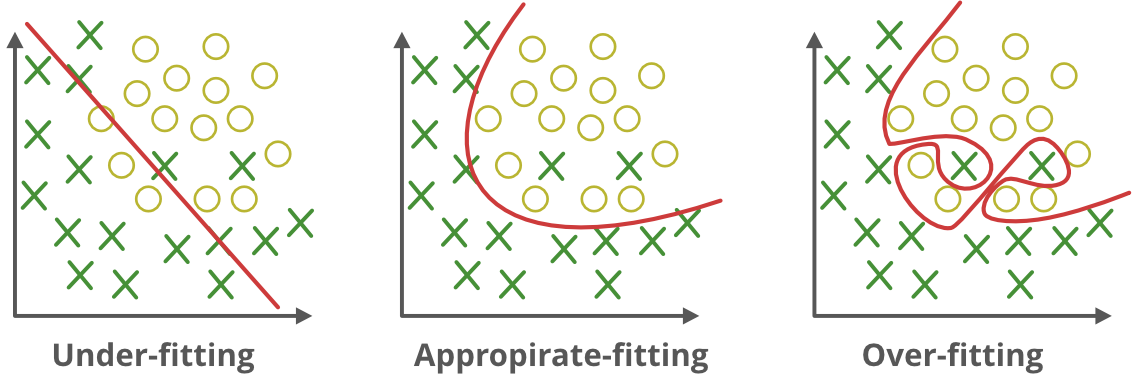
\includegraphics[width=0.65\linewidth]{./source/images/fittingtypes.png}}
  \caption{Typen von Generalisierungseffekten \cite{EDPOJ}.}
  \label{pic:FittingTypes}
\end{figure}
\newpage


\section{Architekturen}
\noindent
Um mithilfe neuronaler Netze die \ac{ATS} zu modellieren, werden nun ausgewählte Architekturen vorgestellt. Diese gehen weit über die als Grundlage beschriebenen \ac{MLP} hinaus und verdeutlichen die Varietät neuronaler Netze.


\subsection{Recurrent Neural Networks}
\noindent
Eingangsdaten der \ac{ATS} haben in jedem Fall einen Textcharakter. Hierbei ist die Reihenfolge der Wörter hinsichtlich eines ausreichenden Textverständnisses von großer Bedeutung. Dies gilt sowohl für die Texte selbst als auch für die darin enthaltenen Sätze. Daher werden nun \ac{RNN} vorgestellt, welche derart sequenzielle Daten mithilfe von zahlreichen verborgenen Zuständen in verborgenen Schichten verarbeiten können \cite[S.~301]{ZHA20}.\\

\noindent
Sei $h_t$ ein solcher verborgener Zustand und $x_t$ ein Wort der Eingabesequenz an einem Index $t > 0$. Der Index ist hierbei als Position eines Wortes innerhalb eines Textes zu verstehen \cite{VAS17}. \ac{RNN} können hierfür die Wahrscheinlichkeit $$P(x_t \mid x_{t-1}, ... , x_1) \approx P(x_t \mid h_{t-1})$$ modellieren. Der verborgene Zustand $h_t$ kann unter Kenntnis des Wortes $x_t$ und des verborgenen Zustandes $h_{t-1}$ gemäß der daraus herleitbaren Funktion $$h_t = f(x_t, h_{t-1})$$ berechnet werden. Letzterer verfügt über die sequenziellen Informationen bis zum Index $t-1$. Weiterhin ist erkennbar, dass die gegebene Funktion der Markoveigenschaft gerecht wird \cite[S.~323-324]{ZHA20}.\\

\noindent
\autoref{pic:HiddenStates} demonstriert den rechentechnischen Vorgang anhand von drei prototypischen verborgenen Zuständen unter gegebenen Eingangsdaten. Wie bereits bei der oben genannten Funktion ersichtlich wurde, gehen in einen verborgenen Zustand jeweils das momentane Wort und der vorhergegangene verborgene Zustand ein. Innerhalb eines verborgenen Zustandes werden diese beiden Eingangsgrößen mithilfe einer Aktivierungsfunktion in eine vollvermaschte Schicht überführt. Zudem wird die Ausgabeschicht mit dem momentanen Output versorgt \cite[S.~325]{ZHA20}. Allgemein haben \ac{RNN} also die Form einer Kette, in der Module neuronaler Netze immer wiederkehren \cite{AIU19}.

\begin{figure}[h!]
  \centering
  \fbox{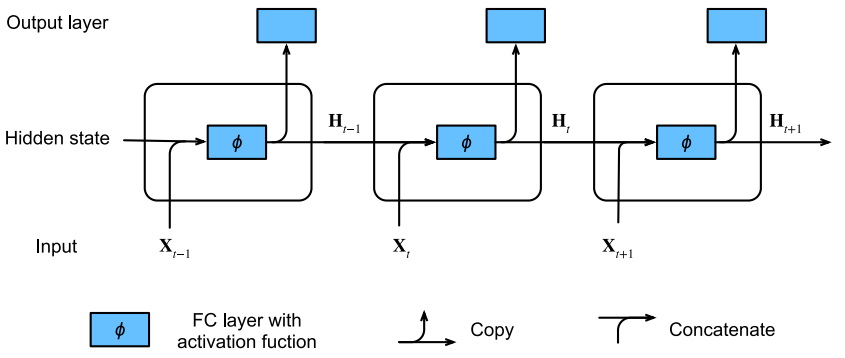
\includegraphics[width=0.8\linewidth]{./source/images/hiddenstates.png}}
  \caption{RNN mit verborgenen Zuständen \cite[S.~325]{ZHA20}.}
  \label{pic:HiddenStates}
\end{figure}

\noindent
Die bereits bekannte beidseitige Propagation ist auch bei \ac{RNN} erforderlich, damit der Trainingsprozess zu einem entsprechenden Lernfortschritt führt. Während die vorwärtige Propagation den oben beschriebenen Prinzipien nachkommt, wird die Backpropagation nun über die Indizes hinweg durchgeführt (engl. Backpropagation Through Time). Bei einer langen Eingabesequenz gehen entsprechend hochdimensionale Matrizen in die Berechnung ein. Dies ist sowohl aus rechentechnischer als auch aus numerischer Sicht nachteilig. Die Anzahl modellinterner Parameter steigt bei steigender Indexanzahl hingegen nicht \cite[S.~328,~340]{ZHA20}.\\

\noindent
Außerdem können \ac{RNN} bidirektional modelliert werden. Die verborgenen Zustände werden demnach stets mit den Werten vor und nach dem momentanen Index berechnet. Diese beidseitige Propagation ist allerdings sehr rechenaufwendig und wird in dieser Arbeit nicht weiter vertieft.\\

\noindent
\ac{RNN} treffen früher oder später auf das Problem verschwindender Gradienten (engl. Vanishing Gradients). Dies tritt insbesondere bei langen Eingabesequenzen auf und führt dazu, dass langfristige Abhängigkeiten nicht mehr gelernt werden können. Die modellinternen Parameter werden im Trainingsprozess bekanntermaßen mithilfe der Backpropagation aktualisiert. Aufgrund fortschreitender Multiplikationen mit Wahrscheinlichkeiten zwischen 0 und 1 werden die Gradienten immer kleiner, bis letztlich kein Lernfortschritt mehr zu verzeichnen ist \cite{ARB18}. Dieses Verhalten kann auch als numerischer Unterlauf bezeichnet werden.\\

\noindent
\ac{LSTM} sind eine Art von \ac{RNN}, welche dazu fähig sind, langfristige Abhängigkeit zu erlernen. Sie vermeiden das Problem verschwindender Gradienten \cite{AIU19}. Außerdem verfolgen sie das Prinzip sogenannter \ac{GRU}. Der entscheidende Mechanismus lässt aus der Funktionsweise von Gates ableiten. Demnach entscheiden diese Gates mit einer Wahrscheinlichkeit zwischen 0 und 1, ob der erhaltene Wert weitergeleitet oder verworfen werden soll. Eine \ac{LSTM}-Zelle verfügt über drei wesentliche Gates: Input Gate, Forget Gate, Output Gate \cite[S.~347-348]{ZHA20}.\\

\noindent
Das Input Gate definiert, welche Werte in der Zelle berücksichtigt werden sollen. Hierzu gehören gemäß \ac{RNN} das momentane Wort sowie der vorhergegangene verborgene Zustand. Das Forget Gate trifft eine Entscheidung darüber, ob und welche Werte gespeichert oder vergessen werden sollen. Hierfür eignen sich beispielsweise Aktivierungsfunktionen \cite[S.~355]{ZHA20}. Über die intern festgelegte Logik kann somit der Zellzustand berechnet werden, unter anderem mithilfe punktweiser Matrixoperationen. Der Zellzustand wird sodann als neuer verborgener Zustand im Output Gate emittiert \cite{LUB18}. Der Aufbau einer \ac{LSTM}-Zelle ist in \autoref{pic:LstmCell} zu sehen.\\

\begin{figure}[h!]
  \centering
  \fbox{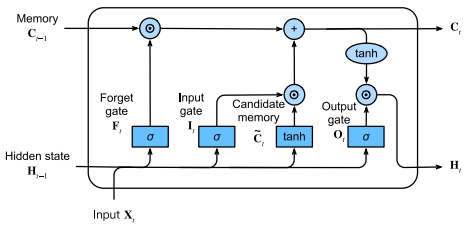
\includegraphics[width=0.7\linewidth]{./source/images/lstmcell.png}}
  \caption{Aufbau einer LSTM-Zelle \cite[S.~357]{ZHA20}.}
  \label{pic:LstmCell}
\end{figure}

\noindent
Ersetzt man die verborgenen Zustände in \autoref{pic:HiddenStates} durch \ac{LSTM}-Zellen, so wird man der beabsichtigten Funktionsweise eines \ac{LSTM} gerecht. Mit fortschreitendem Trainingsprozess werden auch hier sequenzielle Abhängigkeiten gelernt, wobei als irrelevant angenommene Informationen stets verworfen werden. Der Vorteil gegenüber schlichter \ac{RNN} besteht bei den \ac{LSTM} hierdurch insbesondere darin, dass langfristige Abhängigkeiten besonders gut gelernt und bestimmte Informationen schneller gefunden werden können. Dies gilt vor allem für vielschichtige komplexe neuronale Netze, welche anderenfalls unübersichtlich und rechenaufwändig würden \cite{LUB18}.\\

\noindent
Zwar sind \ac{LSTM} den \ac{RNN} qualitativ in vielen \ac{NLP}-Aufgaben überlegen, dennoch sind beide Architekturen eher statistisch getrieben und somit autark als veraltet zu bewerten. Obgleich sie als Grundlage prinzipiell verstanden werden sollten, dominieren maschinelle Lernverfahren qualitativ sowie ressourcentechnisch den \ac{SOTA} mit verschiedenen anderweitigen Architekturen \cite{CUR18}. Diese werden nachfolgend hinreichend erläutert.


\subsection{Encoder-Decoder-Networks}
\noindent
Encoder-Decoder-Architekturen sind zunächst einmal als Template zu verstehen, welches einer stets individuellen Entwicklung und Reife bedarf. Dabei bestehen entsprechende Modelle aus einem Encoder und einem Decoder \cite[S.~375-376]{ZHA20}. Beide Module bestehen de facto aus neuronalen Netzen, welche beispielsweise durch \ac{RNN} oder auch \ac{LSTM} repräsentiert werden können. Hierdurch wird zugleich die Verarbeitung sequenzieller Daten ermöglicht. Hinsichtlich der anvisierten \ac{ATS} spricht man daher auch von Sequence-to-Sequence-Modellen \cite[S.~377]{ZHA20}.\\

\noindent
Im Encoder wird die Eingabesequenz zuerst eingebettet. Hierdurch entsteht ein Merkmalsvektor, welcher entlang eines zugrundeliegenden Wortschatzes aus den Indizes der eingegangenen Wörter besteht. Er ist die mathematisch verarbeitbare Version der Eingabesequenz. Dieser Vorgang wird im weiteren Verlauf dieser Arbeit noch hinreichend beschrieben und untersucht. Der Merkmalsvektor geht sodann in das neuronale Netz des Encoders ein und wird in eine entsprechende Zustandsrepräsentation überführt \cite{YAN19}.\\

\noindent
Der Decoder wird mit den Ausgangsdaten des Encoders initialisiert. Die entsprechende Zustandsrepräsentation wird ebenfalls mithilfe eines neuronalen Netzes verarbeitet \cite[S.379]{ZHA20}. Nun wird jedoch zusätzlich eine Ausgabesequenz generiert, welche der \ac{ATS} gerecht werden soll. Wie bereits bekannt ist, gilt es letztlich die bedingte Wahrscheinlichkeit $P(y \mid x)$ zu modellieren \cite{YAN19}.\\

\noindent
Es folgt nun eine mathematische Betrachtung der Encoder-Decoder-Architektur. Hierfür wird die genannte Zustandsrepräsentation als Kontextvektor $c$ bezeichnet. Die Wahrscheinlichkeit für eine Ausgabe am Index $t > 0$ kann demnach mit $$P(y_t \mid y_1, ..., y_{t-1}, c)$$ modelliert werden. Die Berechnung der verborgenen Zustände im Decoder erfordert nun den Merkmalsvektor, den Kontextvektor und den letzten verborgenen Zustand des Encoders. Hiermit kann $$h_t = f(y_{t-1}, c, s_{t-1})$$ berechnet werden. Informationen, welche an vorherigen Indizes gespeichert sind, können rekursiv ermittelt werden. Architektonisch ist weiterhin zu beachten, dass die Konfiguration des Encoders der Konfiguration des Decoders gleicht. Dies gilt insbesondere für die Anzahl der verborgenen Schichten \cite[S.~379]{ZHA20}.\\

\noindent
Um die theoretisch und abstrakt beschriebene Architektur zu veranschaulichen, werden die wesentlichen Module nun abschließend in \autoref{pic:EncoderDecoder} visuell in Zusammenhang gebracht. Allgemein gilt: Eine Eingabesequenz $x = [x_{1}, ..., x_{n}]$ wird mithilfe des Encoders zunächst in einen kontinuierlichen Zustandsvektor $z = [z_{1}, ..., z_{n}]$ überführt, bevor der Decoder daraus die Ausgabesequenz $y = [y_{1}, ..., y_{m}]$ generieren kann \cite{VAS17}.\\

\begin{figure}[h!]
  \centering
  \fbox{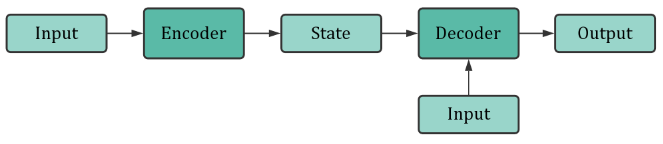
\includegraphics[width=0.7\linewidth]{./source/images/encoderdecoder.png}}
  \caption{Encoder-Decoder-Architektur \cite[S.~375]{ZHA20}.}
  \label{pic:EncoderDecoder}
\end{figure}


\subsection{Attention in Neural Networks}
\noindent
Die Encoder-Decoder-Architektur kann im Kontext der \ac{ATS} um einen sogenannten Attention-Mechanismus erweitert werden, welcher den Encoder mit dem Decoder verbindet \cite{VAS17}. Dabei geht es, wie die Übersetzung schon verrät, um Aufmerksamkeit. In der kognitiven Neurowissenschaft wird Aufmerksamkeit als ein Zustand gesteigerter Anspannung definiert, welcher selektive Wahrnehmung sowie entsprechendes Denken und Handeln umfasst. Diese Fähigkeit wird von einem \ac{ATS}-Modell verlangt und mithilfe des Attention-Mechanismus realisiert. Um letztlich eine qualitative Zusammenfassung generieren zu können, selektiert der Attention-Mechanismus die wichtigsten Informationen aus dem Encoder, indem er die dort verarbeitete Eingabesequenz stets beobachtet und globale Zusammenhänge zwischen der Eingabesequenz und der Ausgabesequenz herstellt. Der Decoder wird dementsprechend darüber informiert. Das \ac{ATS}-Modell soll mathematisch also menschenähnlichem Verhalten nachempfinden, weshalb es per Definition als KI-basierter Ansatz bezeichnet wird \cite[S.~389]{ZHA20}.
\newpage

\noindent
Der Attention-Mechanismus basiert indes auf einer Attention-Funktion, welche eine Query und ein Menge von Key-Value-Paaren einem Output zuordnet. Der Output wird dabei vektorweise als gewichtete Summe der Werte berechnet, während die Query determiniert, welchen Werten mehr Attention zugeordnet wird \cite{VAS17}. \autoref{pic:AttentionLayer} zeigt eine solche Attention-Schicht.\\

\noindent
Die Funktionsweise des Attention-Mechanismus innerhalb einer Encoder-Decoder-Architektur kann nun mithilfe \autoref{pic:AttentionMechanism} weiter vertieft werden, wobei hier Index $t$ betrachtet wird. Dabei bettet der Encoder die Eingabesequenz in bekannter Weise ein und verarbeitet sie, indem die verborgenen Zustände über alle verborgenen Schichten hinweg berechnet werden. Die Attention-Schicht erhält in der Folge alle Informationen, die der Encoder verarbeitet hat. Der Decoder wird nicht nur über den vorangegangenen verborgenen Zustand des Encoders informiert, sondern auch über den aus der Attention-Schicht resultierenden Kontext. Dieser wird als Antwort auf eine Query generiert, wobei eben diese Query wiederum durch den vorangegangenen verborgenen Zustand des Decoders repräsentiert wird \cite[S.~394]{ZHA20}. Die Ausgabesequenz wird hierbei indexweise und autoregressiv generiert, da dem Decoder in jedem Index zusätzlich die bereits generierten Wörter zugeführt werden \cite{VAS17}.\\

\begin{figure}[h!]
  \centering
  \fbox{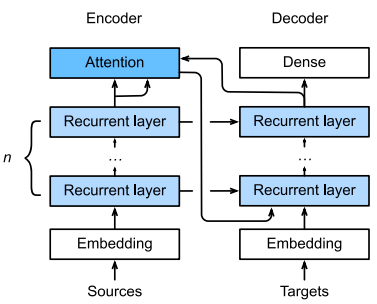
\includegraphics[width=0.55\linewidth]{./source/images/attentionmechanism.png}}
  \caption{Attention-Mechanismus \cite[S.~394]{ZHA20}.}
  \label{pic:AttentionMechanism}
\end{figure}

\noindent
Weiterhin wird zwischen zwei Eigenarten unterschieden: Self-Attention und Multi-Head-Attention. Self-Attention transformiert innerhalb einer Query $n$ Inputs in $n$ Outputs. Dabei interagieren alle Inputs miteinander, um die Verteilung der globalen Attention zu bestimmen. Die Outputs entstehen folglich, indem die entsprechenden Scores aggregiert werden. Betrachtet man also einen Satz, dann ist die Attention jedes darin enthaltenen Wortes zu berechnen \cite{KAR19}. \autoref{pic:SelfAttention} visualisiert die Self-Attention architektonisch.

\begin{figure}[h!]
  \centering
  \fbox{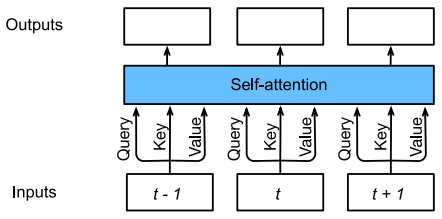
\includegraphics[width=0.5\linewidth]{./source/images/selfattention.png}}
  \caption{Self-Attention \cite[S.~400]{ZHA20}.}
  \label{pic:SelfAttention}
\end{figure}

\noindent
Multi-Head-Attention hingegen betrachtet direkt mehrere Queries. Die Matrizen der Queries Q, Keys K und Values V werden mithilfe entsprechender Gewichtsmatrizen dimensional reduziert, um $$Head = Attention(QW^Q, KW^K, VW^V)$$ zu berechnen. Diese Berechnung geschieht h-mal, sodass entsprechend viele Heads in Form von Gewichtsmatrizen entstehen. Diese werden konkateniert und wiederum mit entsprechenden Gewichtsmatrizen transformiert, sodass $$MultiHead(Q,K,V) = Concat(Head_1, ..., Head_h) \cdot W^O$$ gilt. Hierdurch wird es dem Modell ermöglicht, Informationen aus verschiedenen Repräsentationen zu identifizieren. Betrachtet man also erneut einen Satz, dann werden die Informationen positionsunabhängig und satzübergreifend identifiziert \cite{VAS17}. \autoref{pic:MultiHeadAttention} visualisiert die Multi-Head-Attention architektonisch.
\newpage

\begin{figure}[h!]
  \centering
  \fbox{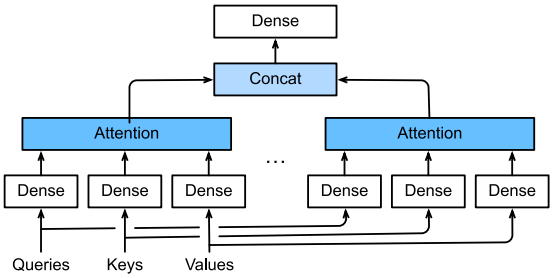
\includegraphics[width=0.7\linewidth]{./source/images/multiheadattention.png}}
  \caption{Multi-Head-Attention \cite[S.~400]{ZHA20}.}
  \label{pic:MultiHeadAttention}
\end{figure}


\subsection{Transformer Networks}
\noindent
Transformer basieren ebenfalls auf der Encoder-Decoder-Architektur, wobei darüber hinaus verschiedene Attention-Mechanismen implementiert werden. Besonders ist hierbei, dass die Eingabesequenz parallel zur Anwendung der Attention-Mechanismen positionsabhängig eingebettet wird, um sequenzielle Informationen zu extrahieren. Dies führt insgesamt zu einem recht kompatiblen Modell, welches nur noch einer stark verringerten Trainingszeit bedarf \cite[S.~398]{ZHA20}.\\

\noindent
Architektonisch werden die rekurrenten Schichten bisheriger Sequence-to-Sequence-Modelle durch Transformer-Module ersetzt. Diese bestehen aus einer Multi-Head-Attention-Schicht, einem positionsabhängigen Feed-Forward-Netzwerk und einer Layer-Normalization-Schicht. Eben diese wird benötigt, um für das entsprechende Modell einen generalisierenden Effekt zu erzielen. Transformer-Module analysieren die eingehenden Wörter unabhängig voneinander. Daher ist es wichtig, die Eingabesequenz positionsabhängig einzubetten, wie oben bereits angedeutet wurde. Hierdurch können sequenzielle Informationen extrahiert werden. Dabei werden überdies keine neuen Abhängigkeiten erlernt, wohl aber die Trainingszeit weiter reduziert \cite[S.~399-404]{ZHA20}. \autoref{pic:TransformerArchitecture} visualisiert die Architektur im Vergleich zu \autoref{pic:AttentionMechanism}.
\newpage

\begin{figure}[h!]
  \centering
  \fbox{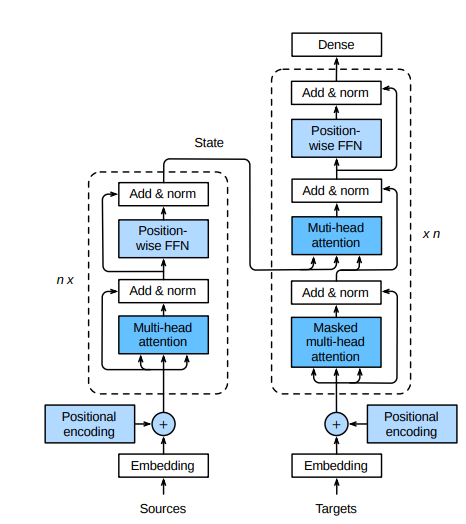
\includegraphics[width=0.65\linewidth]{./source/images/transformerarchitecture.png}}
  \caption{Transformer-Architektur \cite[S.~399]{ZHA20}.}
  \label{pic:TransformerArchitecture}
\end{figure}

\noindent
Zuletzt ist wichtig, dass Transformer und ihre Komponenten verschiedenartig konzipiert werden können. Dies wird stets durch das anvisierte Ziel bedingt. Eine hinsichtlich der \ac{ATS} geeignete Architektur wird in einem entsprechenden Kapitel noch umfangreicher offengelegt. Zudem können bestimmte Komponenten der Transformer durch vortrainierte Modelle repräsentiert werden. Dies wird ebenfalls im weiteren Verlauf dieser Arbeit thematisiert, nachdem entsprechende Grundlagen dargelegt wurden.
\newpage


\section{Hyperparameter}
\noindent
Hyperparameter sind Parameter einer Architektur, die bereits vor dem eigentlichen Trainingsprozess definiert werden. Sie bedürfen einer separaten Optimierung, da sie eben dieses Training und folglich auch die Qualität des entstehenden Modells enorm beeinflussen. Ziel ist es hierbei, die beste Kombination aller Hyperparameter zu finden, um die Fehlerfunktion hinreichend zu minimieren \cite[S.~1]{YAN20}.\\

\noindent
Dies wird im Trainingsprozess als Teil der Backpropagation durch das Gradientenverfahren erreicht, welches die methodische Lösung allgemeiner Optimierungsprobleme übernimmt. Entlang eines negativen Gradienten wird das globale Minimum der dazugehörigen Fehlerfunktion gesucht, bis keine numerische Verbesserung mehr zu verzeichnen ist \cite[S.~428]{ZHA20}. Im weiteren Verlauf werden ausgewählte Hyperparameter, welche das Gradientenverfahren und damit den allgemeinen Trainingsprozess hochgradig beeinflussen, mehr oder minder tiefgründig vorgestellt.\\

\noindent
Die \ac{LR} ist ein Hyperparameter, der bestimmt, wie viel Einfluss jede einzelne Epoche im Trainingsprozess auf die Anpassung der Gewichte nimmt. Sie gilt mithin als wichtigster Hyperparameter einer Architektur \cite[S.~428]{ZHA20}. Eine zu niedrige \ac{LR} kann den Trainingsprozess entweder stark verlangsamen oder dafür sorgen, dass kein Lernfortschritt mehr erzielt wird, da lokale Minima der Fehlerfunktion nicht übersprungen werden können und fälschlicherweise als globales Minimum interpretiert werden. Eine zu hohe \ac{LR} kann hingegen sehr abrupte Anpassungen der Gewichte verursachen, sodass potenziell auch das globale Minimum übersprungen werden kann \cite[S.~414-415]{ZHA20}. \autoref{pic:GradientDescent} verdeutlicht diese Bedingungen. Ziel ist allgemein eine möglichst schnelle Konvergenz.\\

\begin{figure}[h!]
  \centering
  \fbox{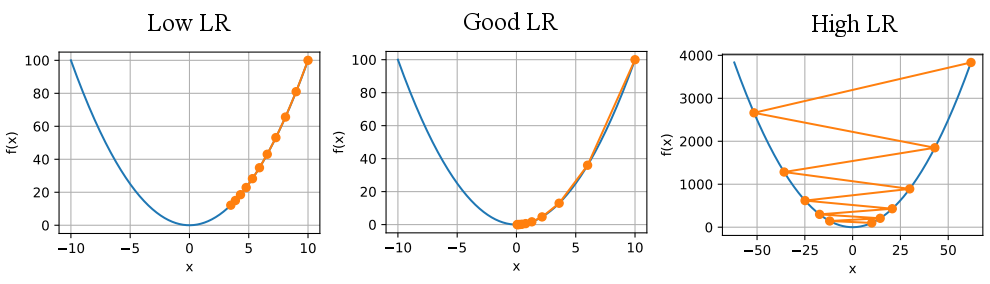
\includegraphics[width=0.65\linewidth]{./source/images/gradientdescent.png}}
  \caption{Konvergenzverhalten im Gradientenverfahren \cite[S.~429]{ZHA20}.}
  \label{pic:GradientDescent}
\end{figure}
\newpage

\noindent
Neben der sorgfältigen manuellen Auswahl der \ac{LR}, etwa mithilfe eines sogenannten \ac{LR}-Schedule, ist es weiterhin möglich, eine adaptive \ac{LR} einzuführen. Hierbei wird die \ac{LR} in jeder Epoche verändert. Üblich ist hier eine Reduktion der \ac{LR}, wenn bereits akzeptable Ergebnisse erreicht wurden \cite[S.~433]{ZHA20}.\\

\noindent
Außerdem existiert das stochastische Gradientenverfahren, welches pro Epoche nur eine Stichprobe der verfügbaren Trainingsdaten berücksichtigt und einen generalisierenden Effekt verspricht \cite[S.~437]{ZHA20}. Die Größe der Stichprobe wird üblicherweise als Batch Size bezeichnet und an dieser Stelle nur als weitergehender Hyperparameter genannt \cite[S.~446]{ZHA20}.\\

\noindent
Weiterhin unterstützt das Momentum die bereits beschriebene \ac{LR} auf der Suche nach dem globalen Minimum in der Fehlerfunktion. Dabei berücksichtigt es den Durchschnitt vorheriger Gradienten. Auf dieser Grundlage wird entschieden, in welche Richtung das stochastische Gradientenverfahren weiter absteigen soll, wie \autoref{pic:MomentumUpdate} zeigt. Das Momentum ist somit potenziell in der Lage, lokale Minima zu überspringen und die Suche erst im tatsächlichen globalen Minimum zu beenden \cite[S.~453-456]{ZHA20}.\\

\begin{figure}[h!]
  \centering
  \fbox{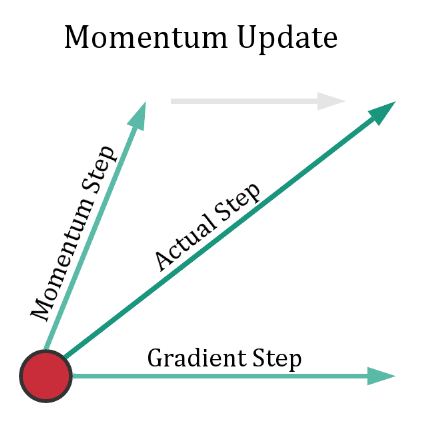
\includegraphics[width=0.3\linewidth]{./source/images/momentumupdate.png}}
  \caption{Gradientenverfahren unter Einfluss eines Momentums \cite{CSNOJ}.}
  \label{pic:MomentumUpdate}
\end{figure}

\noindent
Bei der Auswahl eines hohen Momentums sollte die \ac{LR} eher niedriger sein, oder anders herum. Eine Möglichkeit der stochastischen Optimierung ist hierbei \ac{ADAM}. Dieser Algorithmus übernimmt nicht nur die Auswahl der adaptiven \ac{LR}, sondern auch die Auswahl des entsprechenden Momentums. \ac{ADAM} arbeitet weitreichenden Analysen zufolge effizient für daten- und parameterintensive Probleme. Dabei konvergiert der Algorithmus üblicherweise schneller als vergleichbare Optimierungsalgorithmen \cite[S.~1-2]{KIN17}.\\

\noindent
Zuletzt ist noch das Weight Decay erwähnenswert. Dieses meint die Multiplikation der Gewichte einer Architektur nach jeder Epoche mit einem Faktor kleiner als eins, um sehr große Gewichte zu verhindern. Die Gefahr von Overfitting wird hierbei verringert, während sich die Generalisierung des Modells verbessert \cite[S.~154]{ZHA20}. Allgemein lässt sich die optimale Kombination aller Hyperparameter auch durch Techniken wie Grid Search (vgl. Brute-Force) annähern \cite[S.~24]{YAN20}.


\section{Transfer Learning}
\noindent
\ac{TL} ist in den letzten Jahren wissenschaftlich immer bedeutsamer geworden, da \ac{DL}-Modelle heutzutage sehr komplex und Trainingsprozesse sehr zeit- und rechenintensiv sind. Unter \ac{TL} versteht man das Wiederverwenden bereits vortrainierter neuronaler Netze für die Lösung neuartiger Probleme. Das initiale Training obliegt hierbei meist großen Unternehmen oder Institutionen. Dabei werden die erprobten Modelle sodann als Startpunkt genutzt und nur noch auf die neuen Probleme adaptiert, anstatt eigene Modelle von Grund auf neu zu trainieren. Anwender profitieren hier zeitlich, qualitativ und technisch. Zumeist sind architektonische Anpassungen in den hinteren Schichten der vortrainierten Modelle erforderlich, sodass sie sich für die Lösung der neuen Probleme eignen, wie \autoref{pic:FineTuning} veranschaulicht. Zudem ist ein gezieltes weitergehendes Training mit entsprechenden Daten notwendig. Inwieweit die neuen Daten auf die vortrainierten Modelle einwirken sollen, ist individuell zu erproben \cite[S.~554]{ZHA20}.\\

\begin{figure}[h]
  \centering
  \fbox{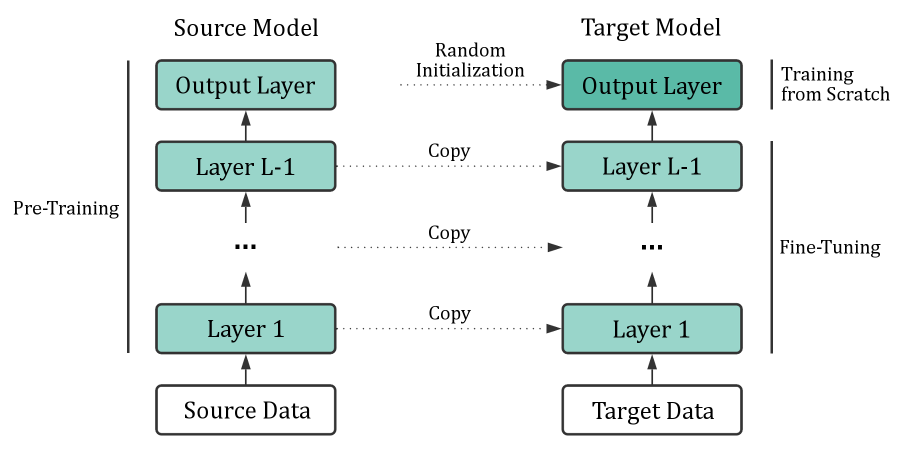
\includegraphics[width=0.7\linewidth]{./source/images/finetuning.png}}
  \caption{Fine-Tuning vortrainierter Modelle \cite[S.~555]{ZHA20}.}
  \label{pic:FineTuning}
\end{figure}
\newpage

\noindent
\ac{TL} wird auch in dieser Arbeit genutzt. Einige Komponenten der bereits vorgestellten Architekturen, wie beispielsweise der Encoder oder auch der Decoder, können durch vortrainierte Modelle repräsentiert werden. Hier wird inhaltlich sowie kontextuell in den folgenden Kapiteln angeknüpft, da zunächst die Einführung weiterer \ac{NLP}-Grundlagen erforderlich ist. Die angeführten Vorteile von \ac{TL} können nichtsdestotrotz folgendermaßen zusammengefasst werden:

\begin{itemize}
	\item Zeitersparnis durch Überspringen des initialen Trainings
	\item Qualitätsanstieg und Generalisierung durch Zuführung massenhafter Daten
	\item Reduktion von Anforderungen, Kosten und Stromverbrauch beim Fine-Tuning
\end{itemize}
